% Template ripped from:
% http://www.cs.technion.ac.il/~yogi/Courses/CS-Scientific-Writing/examples/simple/simple.htm

\title{Differential Privacy with Dependent Types}
\author{
        Casper Holmgreen \\
        Department of Computer Science\\
        DIKU - Datalogisk Institut, K\o benhavns Universitet\\
        \and
        Knut Liest\o l\\
        Department of Computer Science\\
        DIKU - Datalogisk Institut, K\o benhavns Universitet\\
}
\date{\today}

\documentclass[12pt]{article}

\usepackage{graphicx}
\usepackage{listings}
\usepackage{amsfonts,amsthm,amsmath}

\newtheorem{defn}{Definition}[section]

\begin{document}
\maketitle

\lstset{language=Haskell,basicstyle=\footnotesize,frame=single,
        numbers=left}

\begin{abstract}
This is the paper's abstract \ldots
\end{abstract}

\section{Introduction}\label{sec:introduction}

With each passing day, more and more of our personal information is being collected, cataloged and analyzed by an ever increasing number of interested parties.
Their interests can range from targeted advertising to malicious and potentially illegal actions and everything in between.
As the producers of this data, we should be concerned with how it is being used.

[maybe copy paste the rest of this from the original?]

\section{Dependent Types in Idris}\label{sec:dependent_types_in_idris}

Concepts used later in the paper that need to be defined here:
\begin{itemize}
\item Idris data constructors cannot share names with type constructors
\item Very small segment about sections (e.g. \texttt{(*10)})
\item TBD
\end{itemize}

\section{Differential Privacy}\label{sec:differential_privacy}

In this section, we describe the central ideas and metrics behind differential privacy.

\section{Function Sensitivity}\label{sec:function_sensitivity}

Function sensitivity plays a central role in much of the differential privacy literature.
We can make assertions about an entire program if we understand the sensitivities of the functions with which it is composed.
In this section, we describe function sensitivity and then demonstrate how we use dependent types to model it in Idris.

Function sensitivity captures the idea of how relatively ``far'' a function can magnify the distance between pairs of inputs.
We say that a function is $c$-sensitive if, for all pairs of inputs, the distance between the outputs is not $c$ times greater than the original distance between the inputs.

	$$ \forall x,y. d(f(x),f(y)) \le c \times d(x,y) $$

For example, imagine a function $f : \mathbb R \rightarrow \mathbb R$ and Euclidian distance function $d_{\mathbb R}(x,y) = |x-y|$.
Now sample two random values from a 1D line: $x,y$.

Consider the case where $f(x) = \texttt{add10}(x) = x + 10$.
Clearly, it doesn't matter which $x$ and $y$ you sample; the distance $d_{\mathbb R}(x,y)$ will always equal $d_{\mathbb R}(f(x),f(y))$.
We say that \texttt{add10} is a 1-sensitive function.
Now consider the case where $f(x) = \texttt{doubleThenAdd10}(x) = 2x + 10$.
Distances can be now be doubled (but no more), so it is a 2-sensitive function.
Intuitively, when dealing with linear functions and the Euclidian distance function, the largest linear coefficient will dictate the c-sensitivity.
Higher order polynomials can be only be described as being $\infty$-sensitive.

Linear functions and Euclidian distances are not terribly interesting.
Function sensitivity applies to many other interesting domains such as databases containing private tax records or health information.

We will use $\mathbb D$ to describe the domain of databases.
Hence, a function $f : \mathbb D \rightarrow \mathbb D$ is a function across databases.
Our distance function will just be the symmetric difference of two databases; i.e. $d_{\mathbb D}(D_1,D_2) = | D_1 \oplus D_2 |$.
There is a common case in the differential privacy literature where two databases differ by exactly 1 row (i.e. $d_{\mathbb D}(D_1,D_2)=1$).
This is notationally represented by $D_1 \sim D_2$.

Function sensitivies compose, too.
The composition of \texttt{add10 . doubleThenAdd10} is 2-sensitive.
\texttt{doubleThenAdd10 . doubleThenAdd10} is 4-sensitive.
Function sensitivity represents the maximum multiplicative factor by which the distances can increase.
So it follows that the composition of two functions, $f$ and $g$, which are $c$- and $c'$-sensitive, respectively, will be $(c \times c')$-sensitive.

% TODO : discuss any function that is c-sensitive is also c'-sensitive, for all $c < c'$.

\subsection{Function sensitivity in Idris}

Modelling function sensitivity in Idris is simple.
Obviously we will need to index the type by sensitivity.
To keep this example simple, we will use \texttt{Float} to represent it, but our implementation uses an implementation of \texttt{Rational}s, which should be numerically more stable than IEEE floating point numbers.

We define a type constructor indexed by the sensitivity, input and output types, with just one data constructor for wrapping native functions.

\begin{lstlisting}
data SensitiveFunction : Float -> Type -> Type -> Type where
    MkSensitiveFunction : (a -> b) -> SensitiveFunction s a b

namespace Examples

    add10 : SensitiveFunction 1 Float Float
    add10 = MkSensitiveFunction (+10)

    doubleThenAdd10 : SensitiveFunction 2 Float Float
    doubleThenAdd10 = MkSensitiveFunction (*2)

    cheat : SensitiveFunction 1 Float Float
    cheat = MkSensitiveFunction (*20)
\end{lstlisting}

Notice the \texttt{cheat} example above.
It is possible to define so-called ``sensitive functions'' which intentionally misrepresent themselves.
Our focus here is not on the verification of a function's sensitivity, but rather on the interaction between sensitivity and the type system under operations such as function composition or application.
Unrestricted application is as simple as unwrapping the function and applying it.
Composition returns a new data constructor indexed on the appropriate sensitivity.

\begin{lstlisting}
apply : SensitiveFunction s a b -> a -> b
apply (MkSensitiveFunction f) x = f x

(.) : SensitiveFunction s b c -> SensitiveFunction s' a b -> SensitiveFunction (s*s') a c
(.) (MkSensitiveFunction g) (MkSensitiveFunction f) = MkSensitiveFunction (g . f)
\end{lstlisting}
% TODO: Fix text running off page

\section{Typing the Relational Algebra}\label{sec:typing_the_relational_algebra}

In this section, we review the relational algebra and show how it can be modelled in a dependently typed language.
Our approach is based on \cite{OurySwierstra08PowerOfPi}.

The relational algebra describes semantics for modelling and querying data in relational databases (e.g. MySQL\footnote{https://www.mysql.com/}).
E.F. Codd described relational databases and their associated algebra back in the 1970's.
% TODO : find reference to paper
The relational model quickly became popular for its simplicity and good performance.

In the relational algebra, relations are modelled as tables.
The rows of a table represent individual entities and the columns represent their attributes.
Each of these columns is associated with a data type.
Every table has a \textit{schema}, which is the last of its column names and types.
For example, the table below contains four columns; each has a unique name and an associated data type.

\begin{table}[tb]
    \caption{caption here}
    \label{tab:tablename}
    \centering

    \begin{tabular}{|c|c|c|c|}
    \hline

    \hline
    \textbf{Key} & \textbf{Name} & \textbf{Age} & \textbf{FavoriteFood} \\
    \hline
    \textit{Int} & \textit{String} & \textit{Int} & \textit{String} \\
    \hline
    \hline
       1 & Casper & 26 & Chicken Curry \\
       2 & Knut & 26 & ??? \\
       % TODO : Knut fills out fav. food
    \hline

    \end{tabular}
\end{table}

The relational algebra allows us to build structured queries against relational databases.
The primary operators are listed below.
Note that some of the operators may require expressions to be provided (e.g. for filtering a table with a conditional).

\begin{itemize}
    \item selection
    \item projection
    \item Cartesian product\footnote{\label{fn:set_ops} These operations function identically to their set counterparts, but impose additional requirements regarding table schemas. In particular, union and difference (and therefore intersection) require that the schemas of the two operands match. The Cartesian product operator requires that the two schemas are disjoint.}
    \item set union\footnotemark[\ref{fn:set_ops}]
    \item set difference\footnotemark[\ref{fn:set_ops}]
\end{itemize}

Note that the set operations and Cartesian product impose additional requirements in this context.
They have precluded many type systems from being able to fully type-check the relational algebra.
Strongly-typed languages, such as Haskell, have devised clever solutions to this problem, but none are as straight-forward as the approach available to a dependent type system.
The ability to capture schemas directly in the types and to manipulate them yields a deceptively simple, but powerful typing framework for relational databases.

\subsection{Relational Algebra in Idris}

This section will briefly outline a simple implementation of the relational algebra in Idris.
We begin by defining some simple algebraic datatypes (ADTs) for keeping the types clear.
We then define a toy expression language before defining the query language.

First, we need to be able to represent table attributes (columns).
An attribute is just the pairing of a name and a data type.
Following David Christiansen's lead, we opt to use \texttt{(:::)} instead of the more traditional \texttt{(,)} for constructing our pairs.
We believe this enhances readability of long schemas, which are just lists of attributes.

\begin{lstlisting}
data Attribute : Type where
  (:::) : String -> Type -> Attribute

Schema : Type
Schema = List Attribute

namespace Examples

    people : Schema
    people = [ "Key"          ::: Int 
             , "Name"         ::: String
             , "Age"          ::: Int
             , "FavoriteFood" ::: String
             ]
\end{lstlisting}

The relational algebra assumes the existence of an expression language, so we implement a primitive one for demonstration.
An expression will have access to all of the attributes of a row during evaluation and will return a value of some arbitrary type.
Thus, an expression with the type \texttt{Expr s a} can be read as an expression with access to the attributes in schema \texttt{s} returning type \texttt{a}.
Notice that we have not yet defined any underlying representation for the rows.
% TODO : expand on this idea

\begin{figure}[tb]
    \centering
    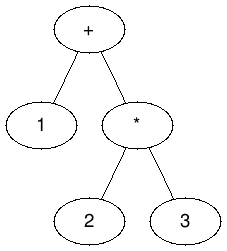
\includegraphics[]{assets/expr_tree.png}
    \caption{Caption here}
    \label{fig:figure1}
\end{figure}
% TODO : resize and work with this graph. write about it in the neighboring text

Expressions can be built up from other expressions, forming an expression tree.
What type will a complex expression tree have?
Expressions cannot change the schema, so it must remain constant even as we grow the tree.
The root of the tree represents the last ``operation'' to be applied under evaluation.
The return type of the root of the tree is the return type of the tree.
Only well-typed expression trees will be allowed by the type checker.

\begin{lstlisting}
data Expr : Schema -> Type -> Type where
    (^)    : (s:Schema) -> (nm:String) -> { auto p : (map cast s) `ContainsKey` nm } -> Expr s (lookupType s p)
    (+)    : Num t => Expr s t -> Expr s t -> Expr s t
    (==)   : Eq t  => Expr s t -> Expr s t -> Expr s Bool
    Lit    : t -> Expr s t
    PureFn : (a -> b) -> Expr s a -> Expr s b

namespace Examples

    fountain_of_youth : Expr s Int
    fountain_of_youth = people^"Age" - 10
\end{lstlisting}

The \texttt{PureFn} data constructor lifts pure Idris functions into the expression language, which should allow programmers to bend even this toy expression language to the task at hand.
Unfortunately, this functionality is only available to the Idris backend.
% TODO: true?
\texttt{ContainsKey} is just a proof that the given schema contains the attribute in question.
It is derived automatically, so users of our language should never have to worry about it.
\texttt{lookupType} is able to use this proof to statically verify the types.

% TODO : insert image of expr AST

The core of the relational algebra consists of the query operators.
They are modelled as follows.
Note that \texttt{Query} is a data family.
This allows us to adjust its data representation just enough to implement a variety of backends.
The leaves of all queries will be very backend specific.
An in-memory Idris backend might store pointers to the tables directly in the data constructor, whereas a SQL backend might just store the name of the table.
One of the benefits of this is that any dataset which can be modelled using the relational algebra is usable.

\begin{lstlisting}
mutual
    data Query : (Schema -> Type) -> Schema -> Type where
        Table   :       t s -> Query t s
        Union   : Query t s -> Query t s -> Query t s
        Diff    : Query t s -> Query t s -> Query t s
        Product : Query t s -> Query t s' -> { auto p : Disjoint s s' } -> Query t (s ++ s')
        Projection : (f:String -> Maybe String) -> Query t s -> Query t (projectedSchema f s)
        Select  : Expr s Bool -> Query t s -> Query t s
    data Grouping : (Schema -> Type) -> Schema -> Type -> Type where
        GroupBy : Eq k => Expr s k -> Query t s -> Grouping t s k
    data Partitioning : (Schema -> Type) -> Schema -> Type -> Type where
        Partition : Eq k => List k -> Expr s k -> Query t s -> Partitioning t s k
\end{lstlisting}

Recall that the set operators require additional constraints that less powerful type systems have a difficult time capturing.
Set union and difference require that the two operands share matching schemas.
Cartesian product requires that they be disjoint.
We just use type unification to express the first two and a machine-decidable proof of disjointness for the other.

% TODO : write about backends

\section{Our implementation}\label{sec:our_implementation}

In this section, we bring together the material of the previous chapters and outline our entire implementation.

\section{Evaluation}\label{sec:evaluation}

In this section, we evaluate our language and discuss various things about it.

\section{Conclusion}\label{sec:conclusion}

We worked very hard, but achieved very little.

\bibliographystyle{abbrv}
\bibliography{main}

\end{document}
